\documentclass[journal,onecolumn]{IEEEtran}

\usepackage[utf8]{inputenc}
\usepackage{fancyhdr}
\usepackage{listings}
\usepackage{geometry}
\usepackage{verbatim}
\usepackage{graphicx}
\usepackage{graphics}
\usepackage{microtype}
\usepackage{listings}
\usepackage{algorithm}
\usepackage{algorithmic}
\usepackage[T1]{fontenc}
% --------------
% --- Título ---
% --------------
\usepackage{titling}
% ---------------
% -- Sections --
% ---------------
\usepackage{titlesec}
\usepackage{sectsty}
\usepackage{pdfpages}
\usepackage{enumitem}

\usepackage{lipsum}
% -----------------
% -- Source code --
% -----------------
\usepackage{listings}
% --------------
% -- Captions --
% --------------
\usepackage{caption}
\usepackage{subcaption}
% ------------------
% -- Bibliografía --
% ------------------
\usepackage{csquotes}

\usepackage{hyperref}
% ---------------------------
% -- Math relatex packages --
% ---------------------------
\usepackage{mathtools}
\usepackage{amssymb}
\usepackage{amssymb}
\usepackage{amsfonts}
\usepackage{amsthm}
\usepackage{physics}
\usepackage{cancel}
\usepackage{cases}
\usepackage{caption}
\usepackage{url}
\usepackage{xurl}
%\usepackage{fouriernc}
\renewcommand\thesection{\roman{section}} 

\renewcommand\thesubsection{\thesection\arabic{subsection}}

%define new section style
\newcommand{\mysection}{
    \titleformat{\section} [runin] {\usefont{OT1}{lmss}{b}{n}}
    {\thesection} {4pt} {} 
}

\geometry{headheight=34.77661pt}


% color def
\definecolor{darkred}{rgb}{0.6,0.0,0.0}
\definecolor{darkgreen}{rgb}{0,0.50,0}
\definecolor{lightblue}{rgb}{0.0,0.42,0.91}
\definecolor{orange}{rgb}{0.99,0.48,0.13}
\definecolor{grass}{rgb}{0.18,0.80,0.18}
\definecolor{pink}{rgb}{0.97,0.15,0.45}

% General Setting of listings
\lstset{
    language=python,
    basicstyle=\ttfamily\small,
    numberstyle=\footnotesize,
    numbers=left,
    backgroundcolor=\color{gray!10},
    frame=single,
    tabsize=4,
    title=\lstname,
    escapeinside={\%*}{*)},
    breaklines=true,
    breakatwhitespace=true,
    framextopmargin=2pt,
    framexbottommargin=2pt,
    inputencoding=utf8,
    extendedchars=true,
    literate={á}{{\'a}}1 {é}{{\'e}}1 {í}{{\'i}}1 {ó}{{\'o}}1 {ú}{{\'u}}1
    {Á}{{\'A}}1 {É}{{\'E}}1 {Í}{{\'I}}1 {Ó}{{\'O}}1 {Ú}{{\'U}}1
    {à}{{\`a}}1 {è}{{\`e}}1 {ì}{{\`i}}1 {ò}{{\`o}}1 {ù}{{\`u}}1
    {À}{{\`A}}1 {È}{{\'E}}1 {Ì}{{\`I}}1 {Ò}{{\`O}}1 {Ù}{{\`U}}1
    {ä}{{\"a}}1 {ë}{{\"e}}1 {ï}{{\"i}}1 {ö}{{\"o}}1 {ü}{{\"u}}1
    {Ä}{{\"A}}1 {Ë}{{\"E}}1 {Ï}{{\"I}}1 {Ö}{{\"O}}1 {Ü}{{\"U}}1
    {â}{{\^a}}1 {ê}{{\^e}}1 {î}{{\^i}}1 {ô}{{\^o}}1 {û}{{\^u}}1
    {Â}{{\^A}}1 {Ê}{{\^E}}1 {Î}{{\^I}}1 {Ô}{{\^O}}1 {Û}{{\^U}}1
    {œ}{{\oe}}1 {Œ}{{\OE}}1 {æ}{{\ae}}1 {Æ}{{\AE}}1 {ß}{{\ss}}1
    {ç}{{\c c}}1 {Ç}{{\c C}}1 {ø}{{\o}}1 {å}{{\r a}}1 {Å}{{\r A}}1
    {€}{{\EUR}}1 {£}{{\pounds}}1 {ñ}{{\~n}}1 {ã}{{\~a}}1 {õ}{{\~o}}1
    {ä}{{\"a}}1 {ü}{{\"u}}1 {¡}{{\textexclamdown}}1 {¿}{{\textquestiondown}}1
}

% 0. Basic Color Theme
\lstdefinestyle{colored}{ %
  basicstyle=\ttfamily,
  backgroundcolor=\color{white},
  commentstyle=\color{green}\itshape,
  keywordstyle=\color{blue}\bfseries\itshape,
  stringstyle=\color{red},
}

% 1. General Python Keywords List
\lstdefinelanguage{PythonPlus}[]{Python}{
  morekeywords=[1]{,as,assert,nonlocal,with,yield,self,True,False,None,} % Python builtin
  morekeywords=[2]{,__init__,__add__,__mul__,__div__,__sub__,__call__,__getitem__,__setitem__,__eq__,__ne__,__nonzero__,__rmul__,__radd__,__repr__,__str__,__get__,__truediv__,__pow__,__name__,__future__,__all__,}, % magic methods
  morekeywords=[3]{,object,type,isinstance,copy,deepcopy,zip,enumerate,reversed,list,set,len,dict,tuple,range,xrange,append,execfile,real,imag,reduce,str,repr,}, % common functions
  morekeywords=[4]{,Exception,NameError,IndexError,SyntaxError,TypeError,ValueError,OverflowError,ZeroDivisionError,}, % errors
  morekeywords=[5]{,ode,fsolve,sqrt,exp,sin,cos,arctan,arctan2,arccos,pi, array,norm,solve,dot,arange,isscalar,max,sum,flatten,shape,reshape,find,any,all,abs,plot,linspace,legend,quad,polyval,polyfit,hstack,concatenate,vstack,column_stack,empty,zeros,ones,rand,vander,grid,pcolor,eig,eigs,eigvals,svd,qr,tan,det,logspace,roll,min,mean,cumsum,cumprod,diff,vectorize,lstsq,cla,eye,xlabel,ylabel,squeeze,}, % numpy / math
}

% 3. Extended theme
\lstdefinestyle{colorEX}{
  basicstyle=\ttfamily,
  backgroundcolor=\color{white},
  commentstyle=\color{darkgreen}\slshape,
  keywordstyle=\color{blue}\bfseries\itshape,
  keywordstyle=[2]\color{blue}\bfseries,
  keywordstyle=[3]\color{grass},
  keywordstyle=[4]\color{red},
  keywordstyle=[5]\color{orange},
  stringstyle=\color{darkred},
  emphstyle=\color{pink}\underbar,
}

\lstset{style=colorEx}
\newcommand{\underbset}[2]{\underset{#1}{\underbrace{#2}}}
\newcommand{\ek}[1]{\cfrac{z^{#1}}{#1!}}
\newcommand{\cek}[1]{\cdot\cfrac{z^{#1}}{#1!}}
\newcommand{\seq}[1]{\left\{#1\right\}}
\newcommand{\se}[2]{\left\{#1\right\}_{#2}}
\newcommand{\cc}{\,\,\,\,\,}
\include{symbols}
% Configuración del documento
%--------------------------

\title{
\includegraphics[width=8cm]{figures/uninorte.png}\\[7ex]
Universidad del Norte - División de Ingenierías\\
Programa de Ingeniería de Sistemas\\[5ex]
Asignatura : Algoritmos y Complejidad\\
Laboratorio: Pareja de puntos más cercanos con lista enlazada\\[5ex]}
\author{Profesor: Misael Díaz Maldonado\\Nombre: David Eduardo Díaz de Moya\\[5ex]}
\date{\today}
% --------------------------
% Configuración de la página
% --------------------------
\pagestyle{fancy}
\fancyhf{}
\rhead{Algoritmos y Complejidad}
\lhead{{
\includegraphics[width=4cm]{figures/uninorte.png}}}
\rfoot{\thepage}

\renewcommand{\headrulewidth}{0.1pt}
\renewcommand*\contentsname{Tabla de contenido}

\geometry{left=1in, right=1in, bottom=1in, top=1in}

% -----------------------
% ------ Contenido ------
% -----------------------
\begin{document}
%
\maketitle
%
\clearpage
\tableofcontents
\clearpage
\section{Resumen}
El presente informe presenta los resultados de optimizar un algoritmo encuentra la pareja más cercana en una lista enlazada de puntos aplicando recursividad. Se realizaron experimentos que consisten en la ejecución del programa con conjuntos de datos cuyo tamaño incrementa en potencias de 2 para el algoritmo recursivo y el algoritmo de fuerza bruta o sin optimizar. Los experimentos se repitieron 10 veces y se registó el tamaño del conjunto de datos, las iteraciones y el tiempo de ejecución para ambos algoritmos. Se graficó el promedio de los resultados para cada algoritmo y se comparó su complejidad temporal promedio. Se obtuvo que la complejidad temporal del algoritmo recursivo es mucho menor a la del algoritmo de fuerza bruta, siendo el primero rápido incluso para conjuntos de datos de entrada de gran tamaño. También se halló que la implementación con listas enlazadas ralentiza el algoritmo, especialmente para conjuntos grandes de datos.
\section{Introducción}
En ciencias de la computación, la complejidad temporal se define como la cantidad de tiempo que se toma un algoritmo en ejecutarse en función del tamaño del conjunto de datos de entrada \ref{bib1}. Es un factor que permite cuantificar el rendimiento de un programa dependiendo de la cantidad de datos que este debe procesar. Para encontrar la complejidad temporal de un programa se cuenta el número de operaciones significativas que el programa realiza para un conjunto de datos de entrada de tamaño N. Generalmente se va a encontrar que el tiempo que un programa se toma no solamente depende de N, sino que tambien puede depender de otros factores del conjunto de datos de entrada. Lo anterior significa que se puede encontrar que un mismo algoritmo puede tardarse diferentes cantidades de tiempo para diferentes conjuntos de datos del mismo tamaño. Diferentes tiempos para conjuntos de datos del mismo tamaño reciben el nombre de casos en el análisis de la complejidad temporal. \ref{bib2}, se tienen en cuenta 3 casos principales:

\begin{enumerate}
    \item El mejor caso o el caso para el cual el tiempo es el menor de todos.
    \item El caso promedio o el promedio de los tiempos de todos los casos.
    \item El peor caso o el caso para el cual el tiempo es el mayor de todos.
\end{enumerate}

El caso promedio será objeto de estudio en el presente informe. Según \ref{bib3}, este está dado por la fórmula: 
\begin{align*}
    A(N) = \cdot \sum_{i=1}^{n} p_i \cdot x_i
\end{align*}
Donde $p_i$ es la posibilidad de que se de el caso $i$ y $x_i$ es la complejidad temporal del mismo caso. Para simplificar el análisis de la complejidad temporal se utiliza la notación asintótica, la cual se deshace de coeficientes y utiliza el término más significativo para representar la complejidad temporal en términos de potencias de N \ref{bib4}. Ejemplo:
\begin{itemize}
    \item $N^0$: El algoritmo siempre se toma la misma cantidad de tiempo, sin importar el tamaño del conjunto de datos de entrada (Tiempo constante).
    \item $N^1$: El número de operaciones que necesita el algoritmo es siempre igual al número de los datos de entrada (Tiempo lineal).
    \item $N^2$: El número de operaciones que necesita el algoritmo incrementa cuadráticamente con respecto al número de los datos de entrada (Tiempo cuadrático).
\end{itemize}
La notación asintótica tiene 3 formas principales:
\begin{itemize}
    \item Big $O$: Describe la complejidad temporal del algoritmo en base al límite superior de esta (Peor caso).
    \item Big $\Omega$: Describe la complejidad temporal del algoritmo en base al límite inferior de esta (Mejor caso).
    \item Big $\Theta$: Describe el orden exacto de la complejidad temporal si está en el mismo orden para todos los casos
\end{itemize}

\section{Planteamiento del Problema}
El rendimiento es uno de los factores más influyentes en la experiencia del usuario al interactuar con software. Consiste principalmente en el tiempo que necesita el programa para responder a algún estímulo o el tiempo que necesita para ejecutar una o varias acciones. Un tiempo de respuesta del programa muy largo puede presentar una molestia al utilizar el programa. Según \ref{bib5}, existen 3 tiempos límites principales a tener en cuenta cuando se habla de desempeño de software:

\begin{enumerate}
    \item 0.1 segundo es el límite para hacer sentir al usuario que el programa está reaccionando instantáneamente.
    \item 1 segundo es el límite para no interrumpir el flujo de trabajo del usuario.
    \item 10 segundos es el límite para mantener la concentración del usuario, si se tiene un tiempo de respuesta mayor a este, el usuario perderá interés en la aplicación.
\end{enumerate}

El rendimiento puede ser incrementado mediante la sustitución de elementos de Hardware por otros con mayores capacidades de procesamiento. Sin embargo, debido a los costos adicionales que esto puede conllevar, es preferible hacer uso de la optimización del Software para mejorar el rendimiento del mismo. La optimización del Software consiste en rediseñar el Software de tal manera que tenga el mismo propósito de antes, sin embargo, que lo logre de una manera más eficiente ya sea necesitando menor espacio temporal en memoria o necesitando una menor cantidad de tiempo para hacer sus operaciones. Uno de los métodos más comunes para la optimización de programas es la división de un problema grande en problemas más pequeños que requieren menos esfuerzo para resolverse. Lo anterior corresponde a la expresión "Divide y vencerás" y en ciencias de la computación frecuentemente se implementa mediante funciones recursivas, las cuales son una forma de diseñar bucles definiendo funciones que se llaman a si mismas hasta que se cumple una condición. Lo anterior se puede utilizar cuando se tienen conjuntos de datos de gran tamaño para analizar ya que permite descartar la mayoría de los datos y solamente analizar un conjunto pequeño. La aplicación más simple de esta forma de optimización es en los algoritmos de búsqueda. El algoritmo de búsqueda lineal recorre todo un arreglo para intentar encontrar un elemento dentro de este. En la figura 1 se puede ver el algoritmo de búsqueda lineal.
\begin{figure}[!htbp]
    \centering
    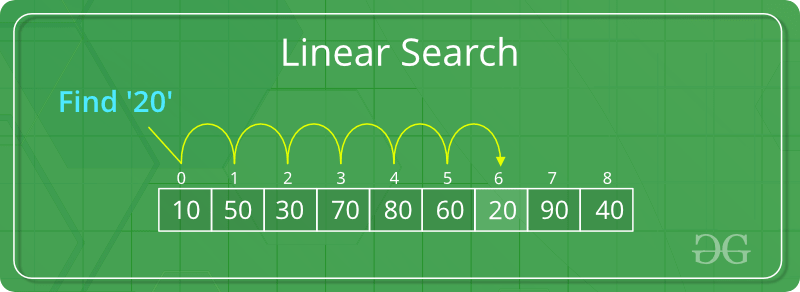
\includegraphics[width=.6\textwidth,height=.3\textwidth]{figures/linear_search.png}
    \caption{Búsqueda lineal \ref{bib6}}
    \label{fig:my_label}
\end{figure}
El rendimiento del algoritmo de búsqueda lineal depende de la posición del elemento que se va a buscar. Si este está en el inicio de la lista, lo encontrará inmediatamente, sin embargo, si este está al final de la lista tendrá que recorrerla toda para encontrar al elemento. En listas de gran tamaño esto significa que el algoritmo puede tomarse una gran cantidad de tiempo. El algoritmo de búsqueda binaria es otro algoritmo de búsqueda que necesita que los elementos de entrada estén ordenados, este algoritmo compara con el elemento central de la lista y si este es menor al elemento que se busca, lo descarta junto con la mitad inferior de la lista, si es mayor, descarta la mitad superior. El algoritmo continúa en la mitad que no se decartó hasta que se encuentre el elemento que se busca. El hecho de que se descarte la mitad de la lista con cada iteración aumenta la velocidad del algoritmo especialmente cuando la lista tiene un tamaño muy grande. En la figura 2 se puede ver el algoritmo de búsqueda binaria.
\begin{figure}[!htbp]
    \centering
    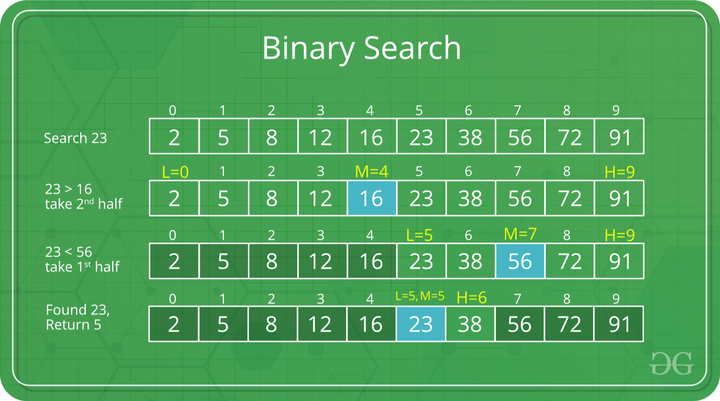
\includegraphics[width=.6\textwidth,height=.4\textwidth]{figures/binary_search.png}
    \caption{Búsqueda binaria \ref{bib7}}
    \label{fig:my_label}
\end{figure}
\section{Metodología}
En esta sección se explicará la metodología y herramientas utilizadas para el desarrollo del presente laboratorio. Se desarrolló un programa en el lenguaje de programación java que dado un conjunto de puntos, encuentra la pareja de puntos que están ubicados a la menor distancia euclideana entre ellos.  Los puntos estarían contenidos en una lista enlazada y estaría ordenados en orden ascendente de acuerdo a su posición. El programa recursivamente divide el conjunto de puntos en pequeños subconjuntos que constan de máximo 3 puntos. Para eso se utiliza una función similar a la que se representa en el siguiente pseudocódigo:

\begin{algorithm}[H]	% uses the float package to control placement
	\caption{Partition(points)}	% a brief description or the function name
	\begin{algorithmic}
	% here is where you use commands from the algorithmic package to
	% write your algorithm
		\IF {$points < 4$}
			\RETURN $Node(points)$
		\ENDIF
		
        \STATE $mid \gets points.len / 2$
        \STATE $half \gets(points.split())$ \COMMENT{Divide la lista en 2 y retorna la otra mitad}
        \STATE $lower \gets$ Partition$(points)$
        \STATE $upper \gets$ Partition$(half)$
        \RETURN $lower.append(upper)$ \COMMENT{Concatenación de listas}
		
	\end{algorithmic}
	\label{algo:factorial}	% defines a label to refer to this
\end{algorithm}

Despues de esto, se ejecuta un algoritmo que compara entre todos los puntos del subconjunto para encontrar la pareja más cercana, este último algoritmo se puede llamar algoritmo de fuerza bruta. El pseudocódigo es el siguiente:

\begin{algorithm}[H]	% uses the float package to control placement
	\caption{BruteForce(points)}	% a brief description or the function name
	\begin{algorithmic}
	% here is where you use commands from the algorithmic package to
	% write your algorithm
	    \STATE $min\_distance \gets LONG\_MAX$
	    \STATE $first \gets points.head()$ \COMMENT{Primer punto de la lista}
	    \WHILE{$first.next() <> null$}
	        \STATE $second \gets first.next$
    	    \WHILE{$second.next() <> null$}
    	        \STATE $d \gets$ distance$(first.data, second.data)$
    	        
    	        \IF{$d < min\_distance$}
    	            \STATE $min\_distance \gets d$
    	        \ENDIF
    	        
    	        \STATE $second \gets second.next$
    	    \ENDWHILE
    	    \STATE $first \gets first.next$
	    \ENDWHILE
	    
    \RETURN $min\_distance$
	\end{algorithmic}
	\label{algo:factorial}	% defines a label to refer to this
\end{algorithm}

Es necesario una función que realice las particiones y ejecute el algoritmo de fuerza bruta sobre cada una de estas, encontrando la distancia mínima entre todas las particiones. Posterior a esto, la función debe comparar a los puntos ubicados en diferentes particiones que puedan ser la pareja más cercana (Si la distancia en x de los dos puntos es menor a la distancia mínima). Para esto, se utilizó el siguiente pseudocódigo:

\begin{algorithm}[H]	% uses the float package to control placement
	\caption{Recursive(points)}	% a brief description or the function name
	\begin{algorithmic}
	% here is where you use commands from the algorithmic package to
	% write your algorithm
	    \STATE $min\_distance \gets LONG\_MAX$
	    \STATE $partitions \gets$ Partition$(partition)$
	    \FOR{each $partition$ in $partitions$}
	        \STATE $d \gets$ BruteForce$(points)$
	        
    	    \IF{$d < min\_distance$}
	            \STATE $min\_distance \gets d$
	        \ENDIF
	    \ENDFOR
	    \STATE $current \gets partitions.head$
	    \WHILE{$current.next <> null$}
	        \STATE $next \gets current.next$
	        \STATE $candidates \gets$ Points between current and next whose $x\_distance < min\_distance$
	        \STATE $d \gets$ BruteForce$(candidates)$
	        \IF{$d < min\_distance$}
	            \STATE $min\_distance \gets d$
	        \ENDIF
	    \ENDWHILE
    \RETURN $min\_distance$
	\end{algorithmic}
	\label{algo:factorial}	% defines a label to refer to this
\end{algorithm}

El programa desarrollado incluye un conteo del número de iteraciones realizado entre el proceso de particionar el conjunto de puntos y comparar las distancias entre puntos, lo cual serviría como resultados para el presente informe. Se realizarían experimentos haciendo uso del algoritmo recursivo como primer caso y del algoritmo de fuerza bruta en todo el conjunto de datos como segundo caso, lo anterior es para comparar las mejoras en la complejidad temporal que representa el uso del algoritmo recursivo con respecto al algoritmo de fuerza bruta. Los experimentos se realizarían con conjuntos de datos cuyo tamaño incrementa en potencias de 2 entre $2^1$ y $2^16$, repitiéndose 10 veces para cada tamaño del conjunto de datos de entrada. Los resultados se escribirían junto con el promedio de las 10 repeticiones, en un archivo de texto tabular cuyo delimitador son los espacios. Posteriormente se tomaron estos resultados obtenidos y se graficaron de forma logarítmica haciendo uso de la librería matplotlib del lenguaje de programación Python. Los resultados obtenidos serían contrastados con los de la implementación con ArrayLists.
\section{Resultados}
En la presente sección se presentarán los resultados de la ejecución de los experimentos planteados. Se presentarán los resultados de forma gráfica para cada uno de los casos a evaluar. Cabe aclarar que aunque se hicieron 10 repeticiones para ambos algoritmos, en esta seción de resultados solamente se va a presentar el promedio de las 10 repeticiones, debido a que el objetivo es mostrar la complejidad temporal promedio. \\


\subsection{Gráficas de resultados}
En la siguiente sección se procesarán los resultados obtenidos anteriormente mediante un programa de python que utiliza la librería Matplotlib para representar los resultados de una manera gráfica. Se mostrará una gráfica logarítmica para cada uno de los algoritmos que mostrará el orden de la complejidad temporal de estos para entradas de distintos tamaños. A continuación en la figura 3 se muestra la gráfica para el algoritmo de fuerza bruta.\\
\begin{figure}[!htbp]
    \centering
    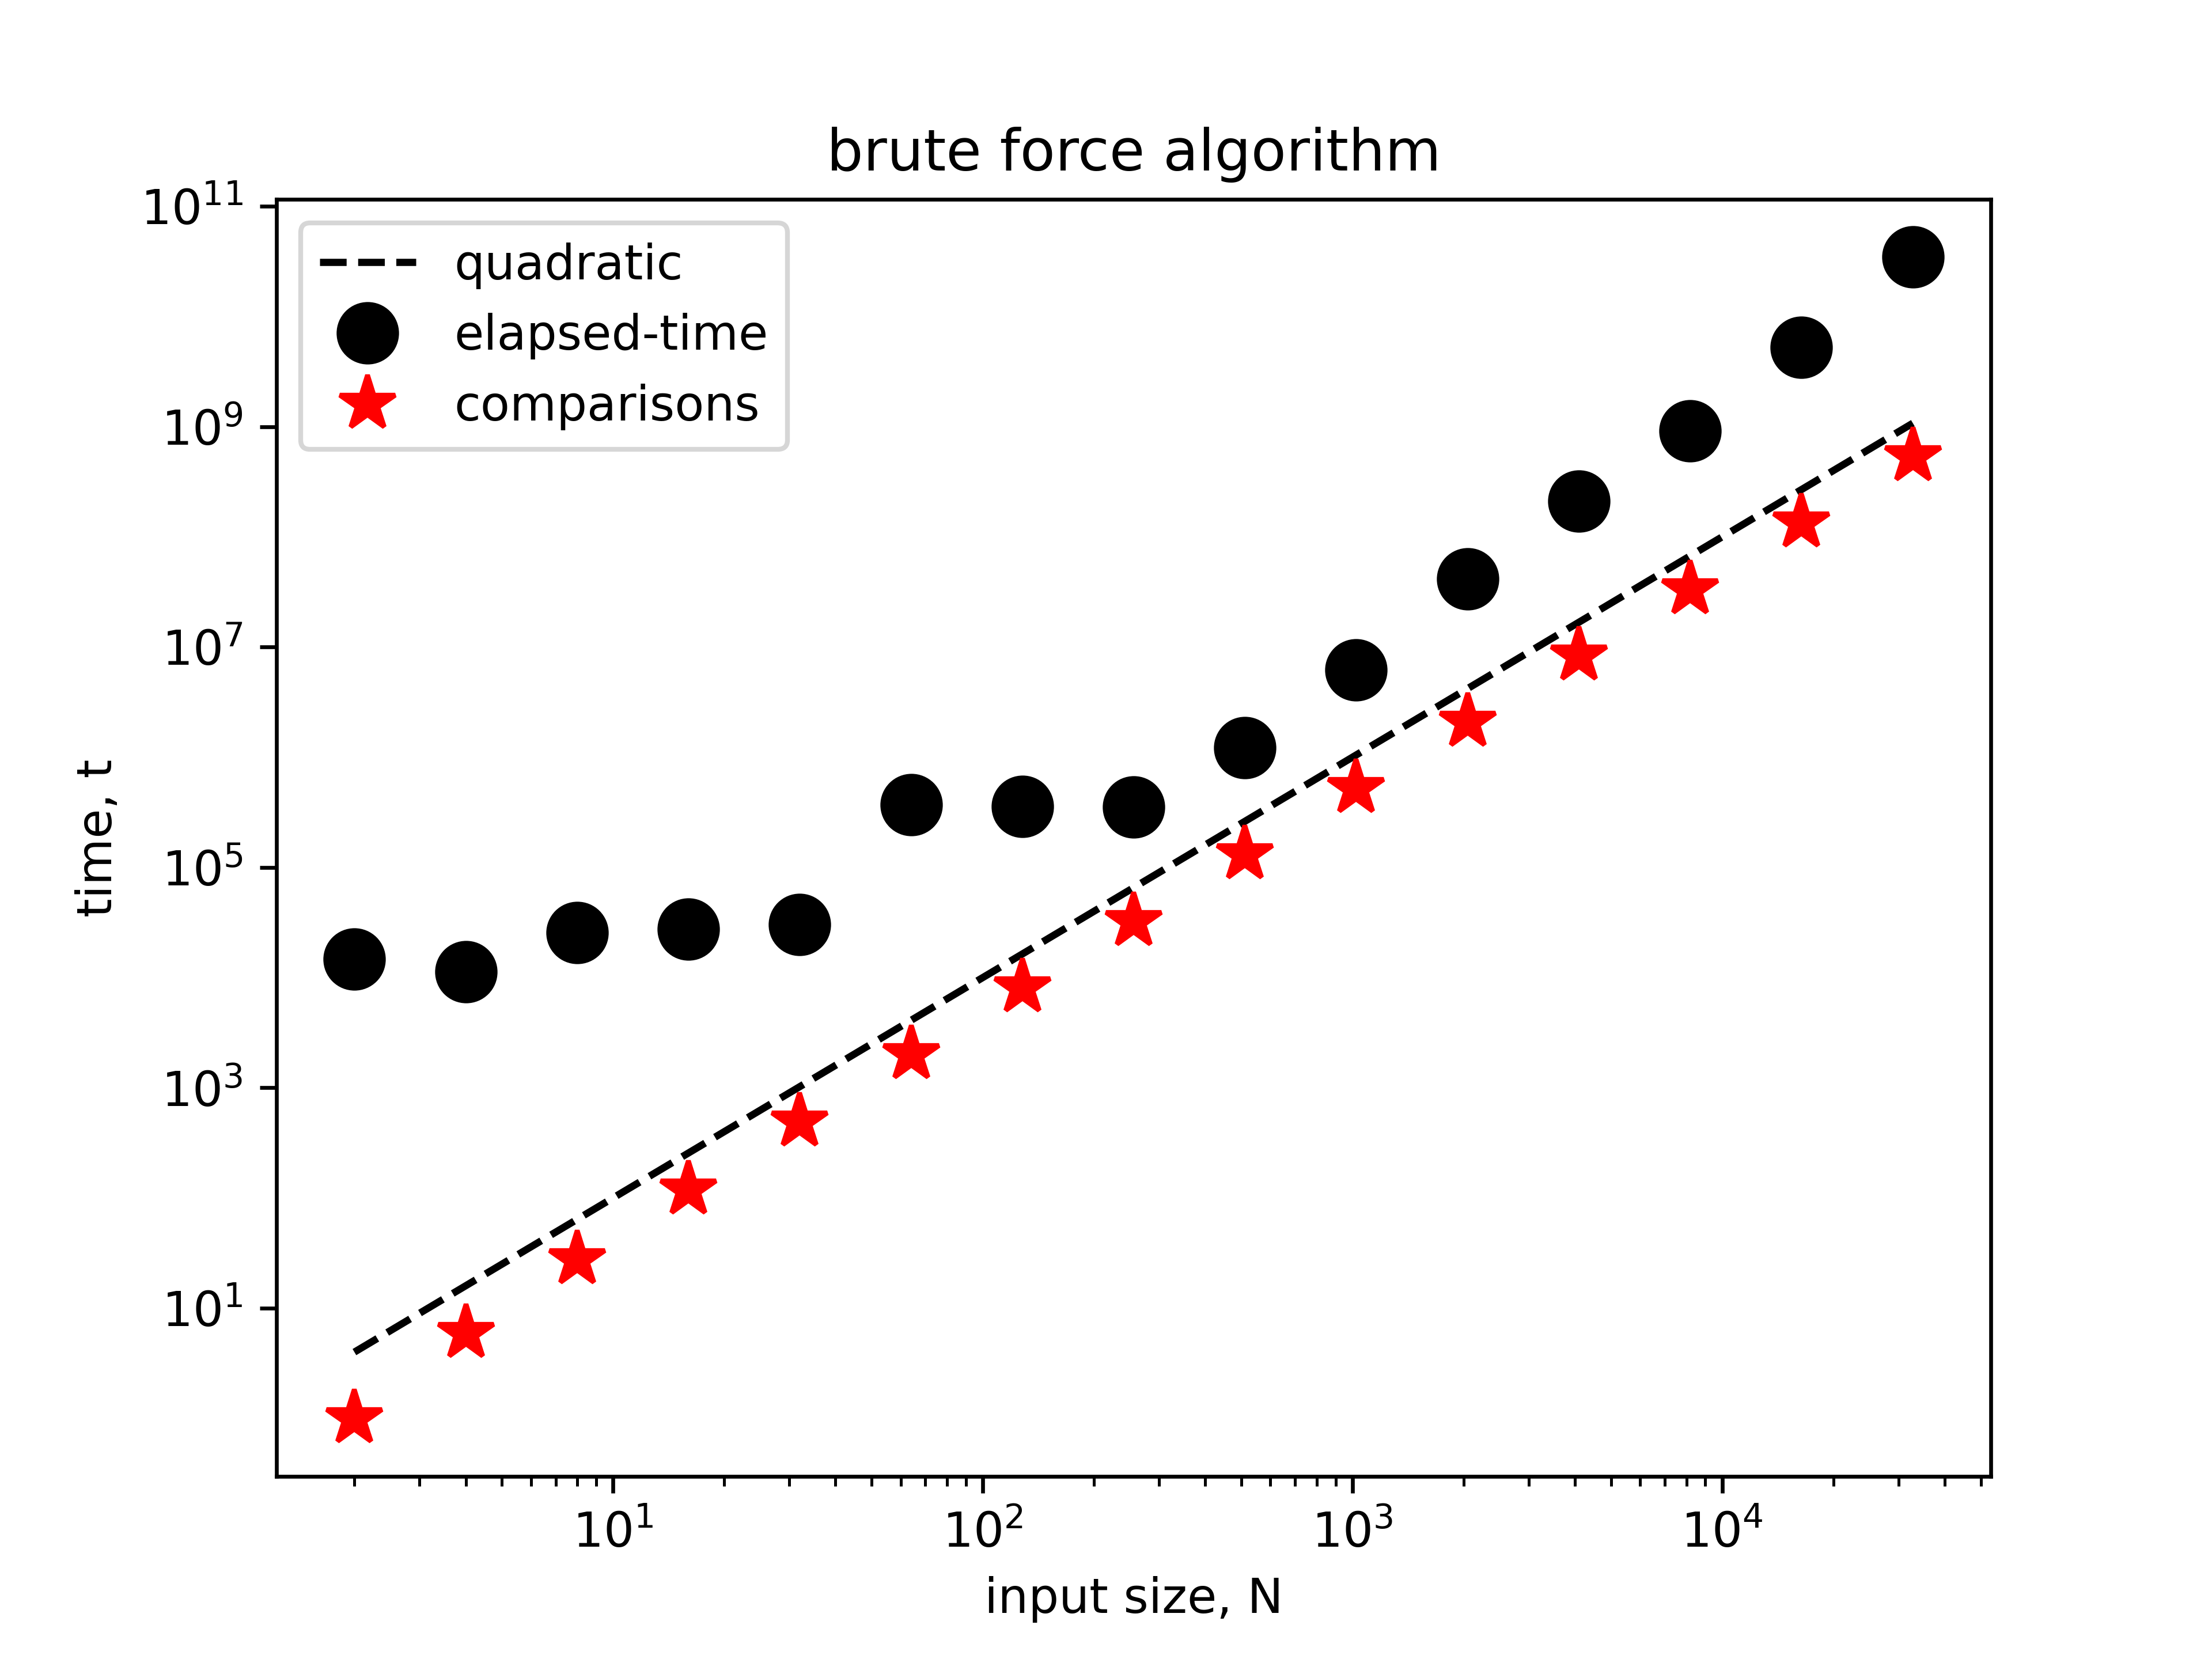
\includegraphics[width=.7\textwidth,height=.5\textwidth]{figures/brute force.png}
    \caption{Gráfica complejidad temporal algoritmo de fuerza bruta}
    \label{fig:my_label}
\end{figure}
La siguiente gráfica es la del algoritmo recursivo. Se puede ver esta en la figura 4.\\
\begin{figure}[!htbp]
    \centering
    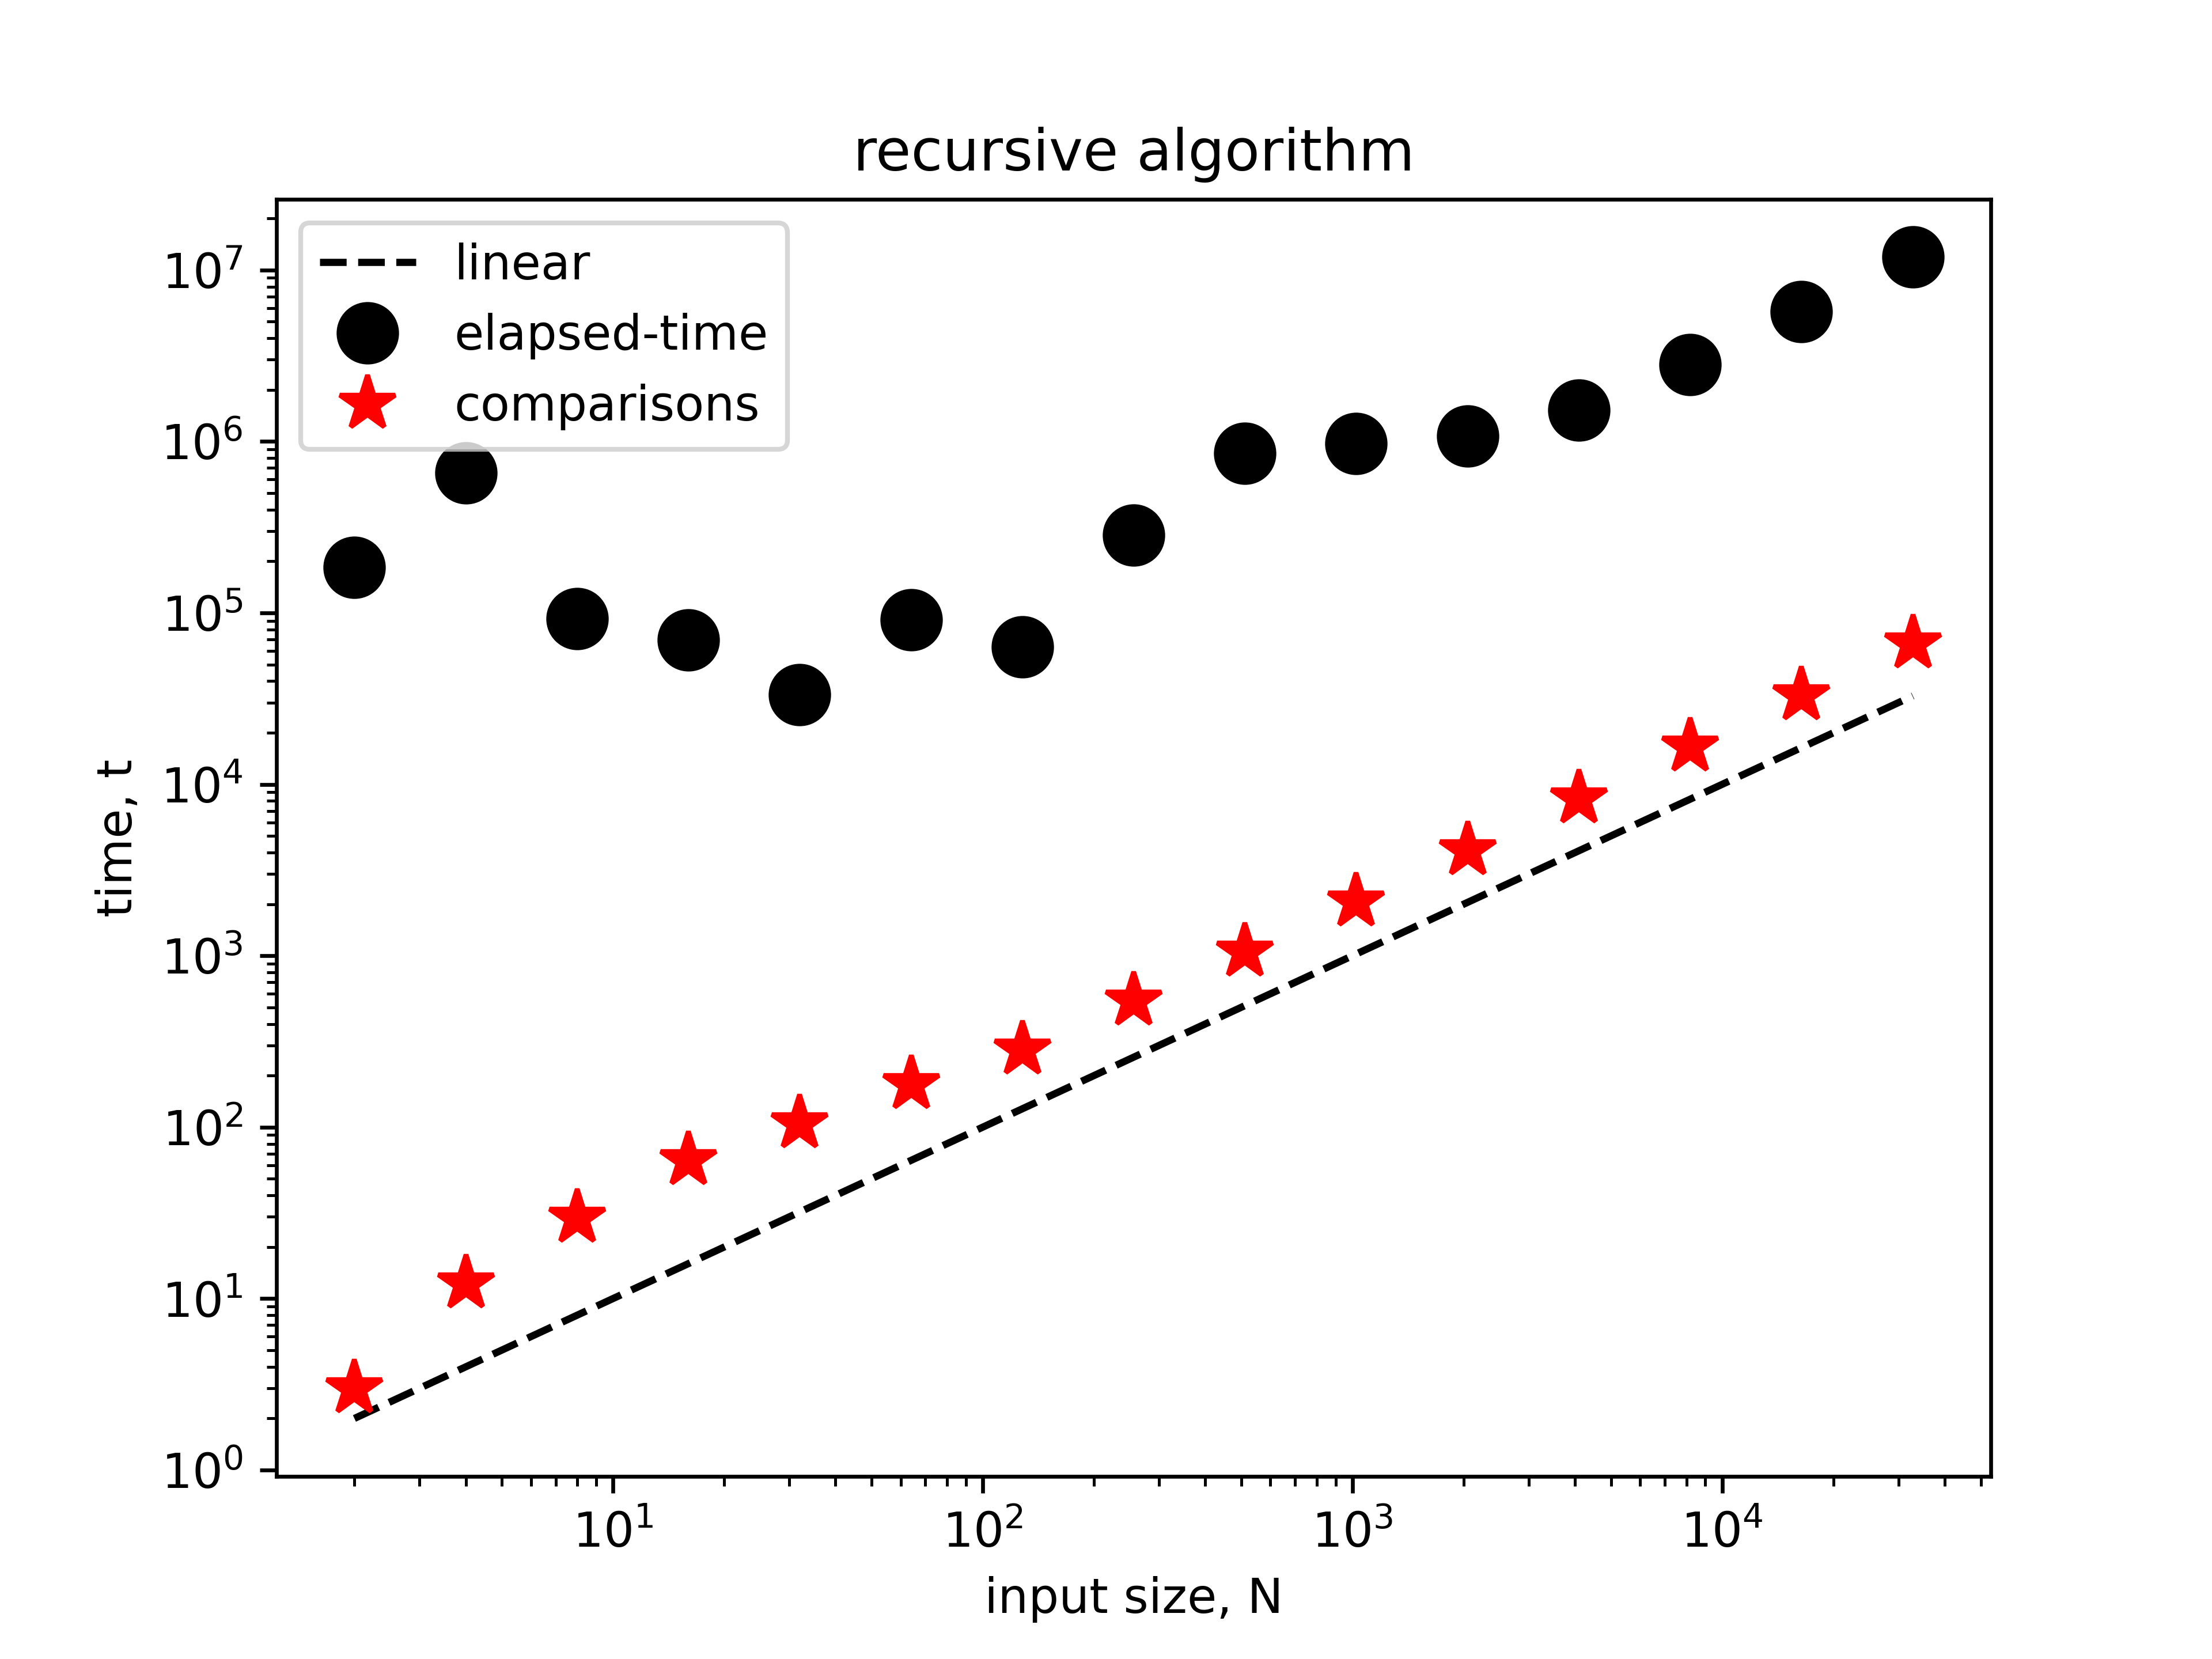
\includegraphics[width=.7\textwidth,height=.5\textwidth]{figures/recursive.png}
    \caption{Gráfica complejidad temporal algoritmo recursivo}
    \label{fig:my_label}
\end{figure}
\section{Análisis de Resultados}

En la presente sección se realizará un análisis de los resultados obtenidos de la parte experimental del laboratorio que se presentaron en la sección anterior. Se verificará que estos resultados concuerden con lo esperado para validar el funcionamiento de ambos algoritmos. La gráfica de los resultados del algoritmo de fuerza bruta se puede ver en la figura 3. Lo que se puede destacar principalmente acerca de estos resultados es un incremento de el número de iteraciones que realizar el algoritmo que aumenta de forma cuadrática cuando incrementa el tamaño del conjunto de datos de entrada. El tiempo transcurrido incrementa de manera cuadrática similar al número de iteraciones. Lo que se puede destacar de estos resultados es que son muy similares a los del la implementación utilizando arraylists. Por otro lado, la figura 4 contiene la gráfica de los resultados del algoritmo recursivo. Para este algoritmo se puede ver que el número de iteraciones que se realizan incrementa en un orden más similar con el linear al incrementar el tamaño del conjunto de datos de entrada. Estas iteraciones incluyen el proceso de dividir recursivamente el conjunto de datos de entrada en varios subconjuntos, ejecutar el algoritmo de fuerza bruta entre los elementos de cada uno de estos conjuntos y de ejecutar el algoritmo de fuerza bruta entre los elementos de 2 diferentes conjuntos que pueden ser la pareja más cercana. Para conjuntos de datos muy pequeños, la diferencia con respecto al algoritmo de fuerza bruta es despreciable, sin embargo, cuando el tamaño del conjunto de datos incrementa, el algoritmo recursivo presenta un desempeño mucho mejor al del algoritmo de fuerza bruta al reducirse el número de comparaciones que se hacen por cada uno de los elementos a una o dos dependiendo del tamaño del subconjunto de datos. Además de lo anterior, al compararse con la implementación realizada con ArrayLists, se puede apreciar que existe una diferencia en el número de comparaciones del algoritmo. En la gráfica del algoritmo recursivo se puede apreciar que el número de comparaciones es mayor en la implementación con listas enlazadas que en la implementación con arraylists, lo anterior se puede justificar en que las listas enlazadas no tienen una forma de acceso aleatorio, por lo cual cuando se quiera acceder a un elemento que no está en la cabeza ni en el final de la lista, es necesario recorrerla secuencialmente, lo anterior puede ralentizar el algoritmo, especialmente en el proceso de particionar la lista, donde es necesario dividir la lista por la mitad hasta que se tenga listas muy pequeñas.
\section{Conclusiones}

Al comparar los resultados obtenidos en esta implementación del algoritmo con los resultados obtenidos de la implementación con ArrayLists, se dijo en la sección de análisis de resultados que se encontraba que el uso de listas enlazadas ralentizaba al algoritmo, lo anterior se debe a que las listas enlazadas solo puede ser accedidas de manera aleatoria. La ralentización es especialmente notoria en el sentido que para procesar la misma cantidad de datos, la implementación con arraylists se tomó cerca de 45 segundos mientras que la implementación con listas enlazadas se tomó mas de 6 minutos. Debido a como se dió la implementación de las listas enlazadas, donde se tiene un campo en el nodo para el dato contenido y un campo para el enlace al siguiente nodo, también existe una mayor cantidad de espacio en memoria principal consumido, donde ahora se requieren 2 campos para contener a un solo dato si se incluye el campo que contiene al enlace. De lo anterior se puede concluir que la implementación con ArrayLists tiene un mejor desempeño que la implementación con listas enlazadas a pesar de que ambas se encuentran en el mismo orden.
\section{Bibliografía}
\begin{enumerate}[label={[\arabic*]}]
  \item \label{bib1} “Time Complexity and Space Complexity,” GeeksforGeeks, 15-Jul-2022. [Online]. Available: \url{https://www.geeksforgeeks.org/time-complexity-and-space-complexity/}. [Accessed: 04-Nov-2022].  
  \item \label{bib2} “Worst, Average and Best Case Analysis of Algorithms,” GeeksforGeeks, Feb. 19, 2012. [Online]. Available: \url{https://www.geeksforgeeks.org/worst-average-and-best-case-analysis-of-algorithms/}. [Accessed: Nov. 04, 2022]
\item \label{bib3} S. Zeil, “Average Case Analysis,” www.cs.odu.edu. [Online]. Available: \url{https://www.cs.odu.edu/~zeil/cs361/latest/Public/averagecase/index.html#determining-the-average-case-complexity}. [Accessed: Nov. 04, 2022]

\item \label{bib4} “Asymptotic notation (article) | Algorithms,” Khan Academy. [Online]. Available: \url{https://www.khanacademy.org/computing/computer-science/algorithms/asymptotic-notation/a/asymptotic-notation}. [Accessed: Nov. 04, 2022]
  \item \label{bib5} Nielsen, Usability engineering. Amsterdam: Morgan Kaufmann, 1993, pp. 115-163.
  \item \label{bib6} “Linear Search - GeeksforGeeks,” GeeksforGeeks, Feb. 2019. [Online]. Available: \url{https://www.geeksforgeeks.org/linear-search/}. [Accessed: Nov. 04, 2022].
  \item \label{bib7} “Binary Search - GeeksforGeeks,” GeeksforGeeks, Apr. 2019. [Online]. Available: \url{https://www.geeksforgeeks.org/binary-search/}. [Accessed: Nov. 04, 2022].
\end{enumerate}

\end{document}